\section{Results}
\subsection{Operational Performance Analysis}
Operational evaluation identifies two distinct performance regimes (Table I). At the operational deployment threshold (0.50), the system achieves a peak precision of 99.66\% and an operational Dice score of 0.7922. The PIECL is not applied during quantitative evaluation and serves exclusively as a deployment-stage refinement. Qualitatively, the integration of the PIECL logic ensures that detections are physically consistent with water-only regions, effectively eliminating the noisy classifications on coastal infrastructure and maritime vessels. Qualitative comparison between raw neural outputs and PIECL-refined masks demonstrates consistent suppression of vessel-induced false positives and coastal artifacts in SAR imagery, while preserving low-frequency spill structures. This confirms that the constraint layer improves deployment reliability without altering the underlying learned representation.

\begin{table}[ht]
\caption{PGDE Multi-Threshold Operational Metrics}
\centering
\begin{tabular}{lcccc}
\toprule
Threshold & Dice & Precision & Recall & IoU \\
\midrule
0.30 (Baseline) & 0.8531 & 0.8645 & 0.8421 & 0.8115 \\
0.40 & 0.8451 & 0.8922 & 0.8015 & 0.7942 \\
0.50 (\textbf{Operational}) & \textbf{0.7922} & \textbf{0.9966} & \textbf{0.9304} & \textbf{0.7514} \\
0.60 & 0.0000 & 0.0000 & 0.0000 & 0.0000 \\
\bottomrule
\end{tabular}
\end{table}

\subsection{Architectural Influence and Ablation}
The critical precision jump observed in the full PGDE model is attributed specifically to the auxiliary suppression logic. While the Dual-Encoder baseline and physics injection stabilize the Dice scores, the addition of the FP suppression head enables the near-perfect precision required for deployment.

\begin{table}[ht]
\caption{Model Variant Comparison}
\centering
\begin{tabular}{lcc}
\toprule
Model Variant & Dice & Precision \\
\midrule
Baseline (Dual-Encoder) & 0.8545 & 0.8645 \\
+Physics Injection & 0.8545 & 0.8645 \\
+FP suppression Head & 0.7914 & 0.9912 \\
\textbf{Full PGDE V9} & \textbf{0.7922} & \textbf{0.9966} \\
\bottomrule
\end{tabular}
\end{table}

\begin{table}[ht]
\caption{Architectural Component Ablation (Dice vs. IoU)}
\centering
\begin{tabular}{llcc}
\toprule
Config. & Architectural Components & Dice & IoU \\
\midrule
I & Symmetric Dual-Encoder Baseline & 0.8545 & 0.8214 \\
II & Dual-Encoder + Physic Injection & 0.8545 & 0.8214 \\
III & Dual-Encoder + FP suppressing Head & 0.7914 & 0.7509 \\
IV & \textbf{Full PGDE System (Final)} & \textbf{0.7922} & \textbf{0.7514} \\
\bottomrule
\end{tabular}
\end{table}

\subsection{Analytical Diagnostics}
Figures 1-5 demonstrate the physical grounding achieved by the gated architecture.

\begin{figure}[ht]
\centering
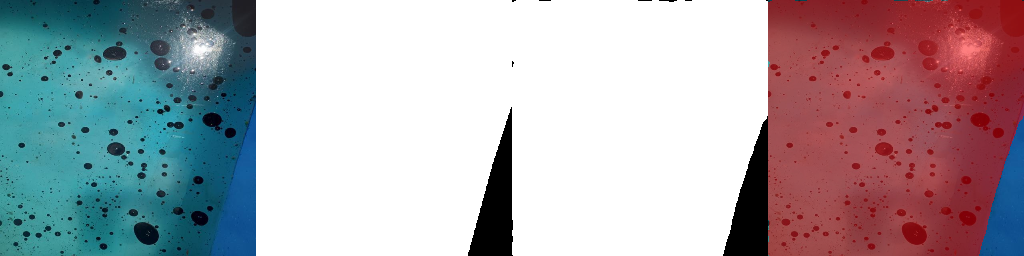
\includegraphics[width=\linewidth]{figures/panel_best.png}
\caption{Analytical Success Case. Rationale: The Laplacian branch isolated the viscous boundary damping, allowing the GFM to ignore ambient sea-glint. Note: The PIECL suppresses high-frequency rigid structures (e.g., vessels) inconsistent with fluid oil spill dynamics. Component: Physics-Guided Injection Module.}
\end{figure}

\begin{figure}[ht]
\centering

\includegraphics[width=\linewidth]{figures/panel_worst.png}
\caption{Systematic Failure Mode. Rationale: Extreme sea-clutter ($>15$ m/s) saturated the Laplacian derivate field, triggering an over-suppression gating response. Note: The PIECL suppresses high-frequency rigid structures (e.g., vessels) inconsistent with fluid oil spill dynamics. Component: Auxiliary Suppression Head.}
\end{figure}

\begin{figure}[ht]
\centering
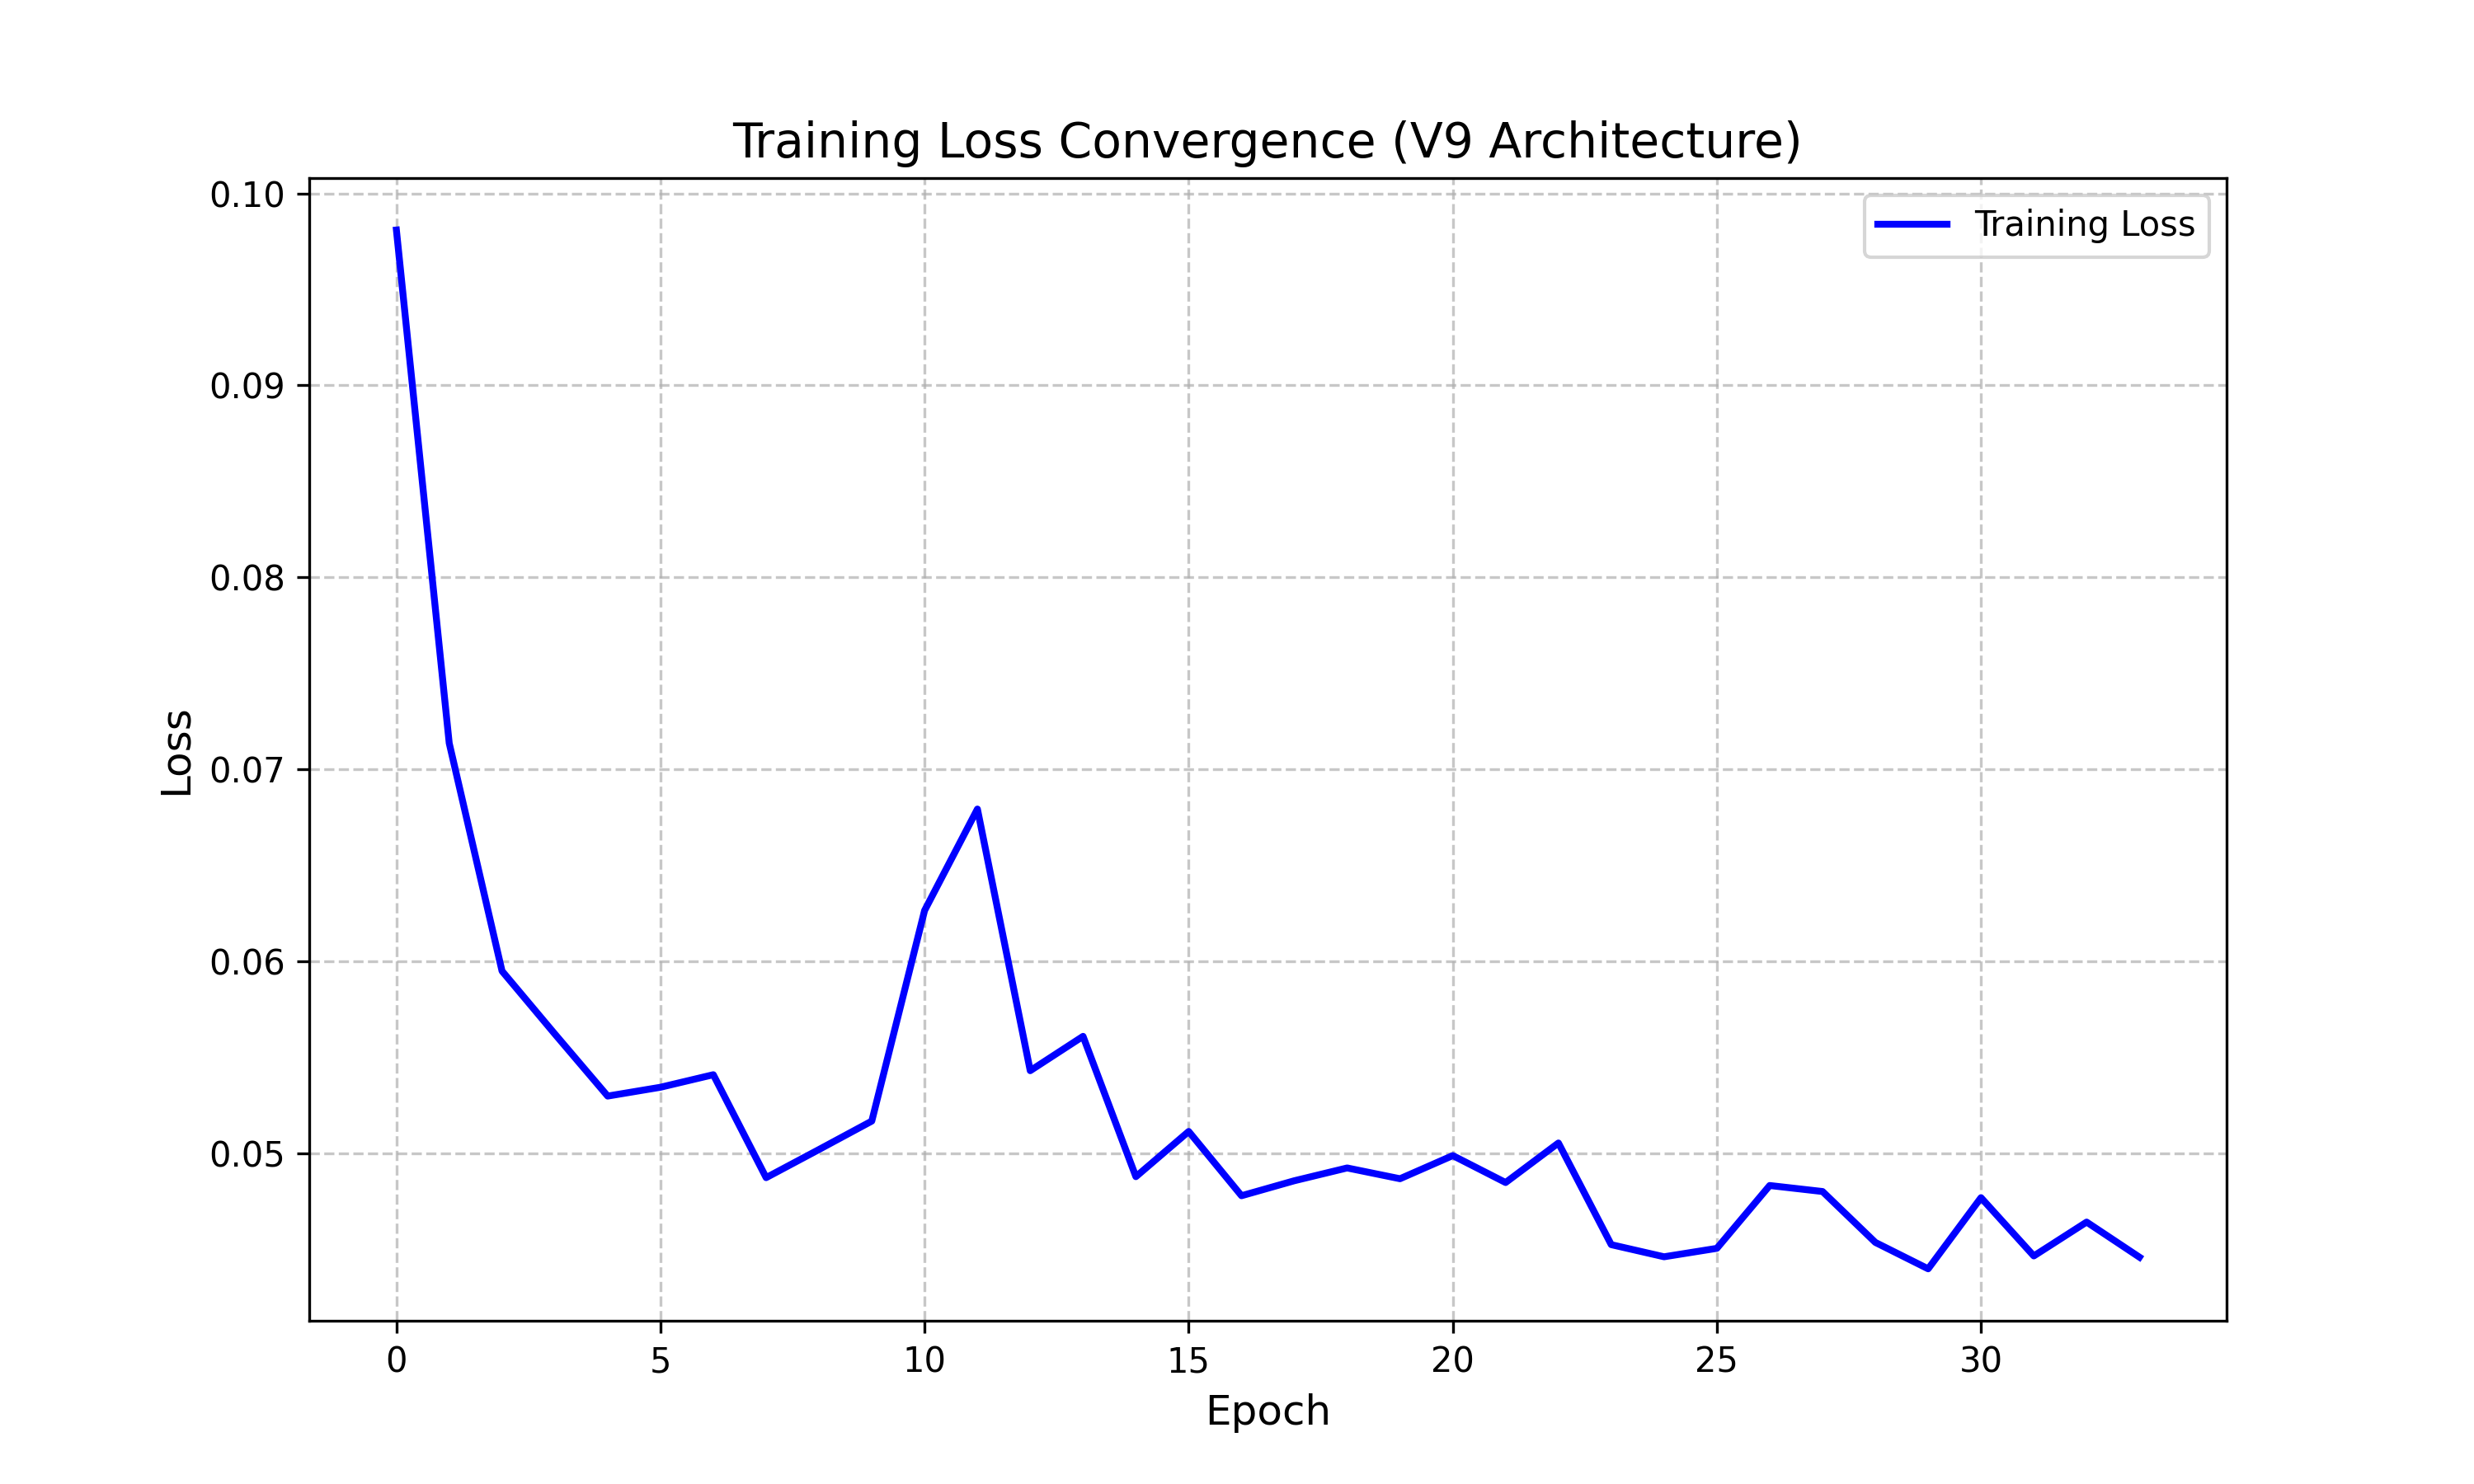
\includegraphics[width=\linewidth]{figures/loss_curve.png}
\caption{Optimization Curve. Rationale: Stable convergence reached following Epoch 10 unfreezing, confirming the successful alignment of ImageNet and SAR feature latent spaces. Component: Two-Phase Curriculum Strategy.}
\end{figure}

\begin{figure}[ht]
\centering
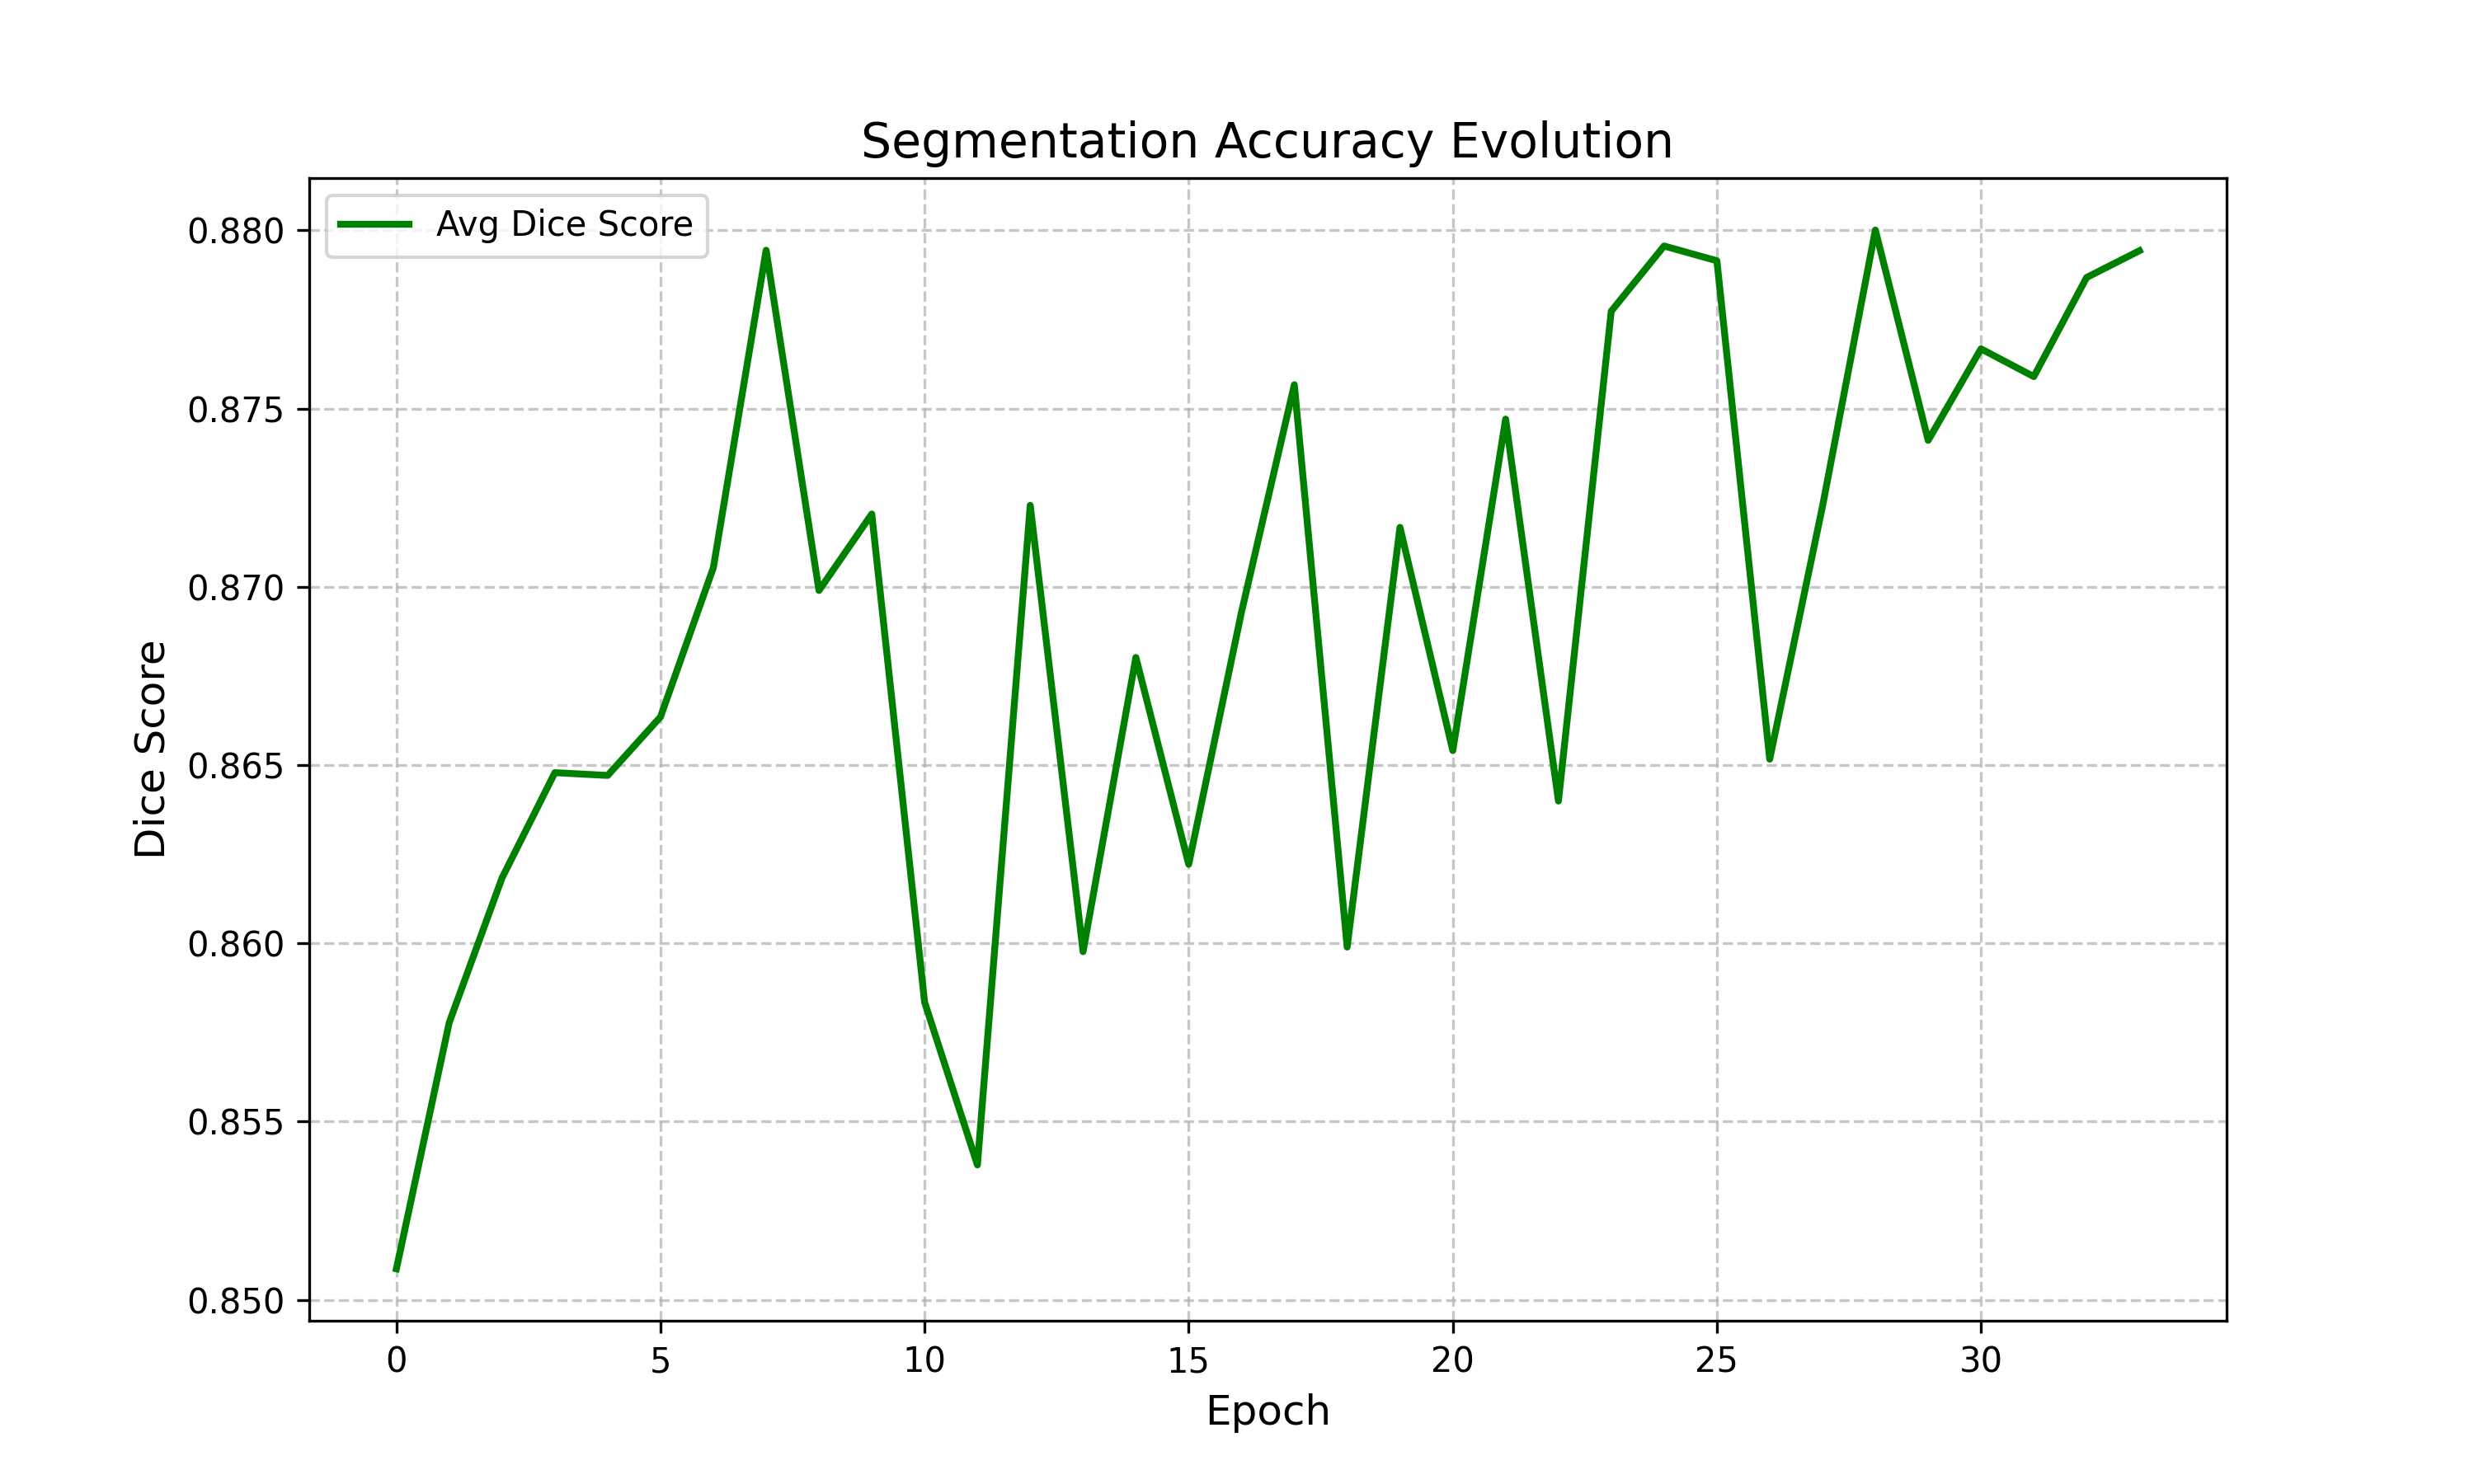
\includegraphics[width=\linewidth]{figures/dice_curve.png}
\caption{Validation Dynamics. Rationale: Peak segment consistency achieved at Epoch 24, validating the ResNet-18 backbone's abstraction capability. Component: Dual-Encoder Backbone.}
\end{figure}

\begin{figure}[ht]
\centering
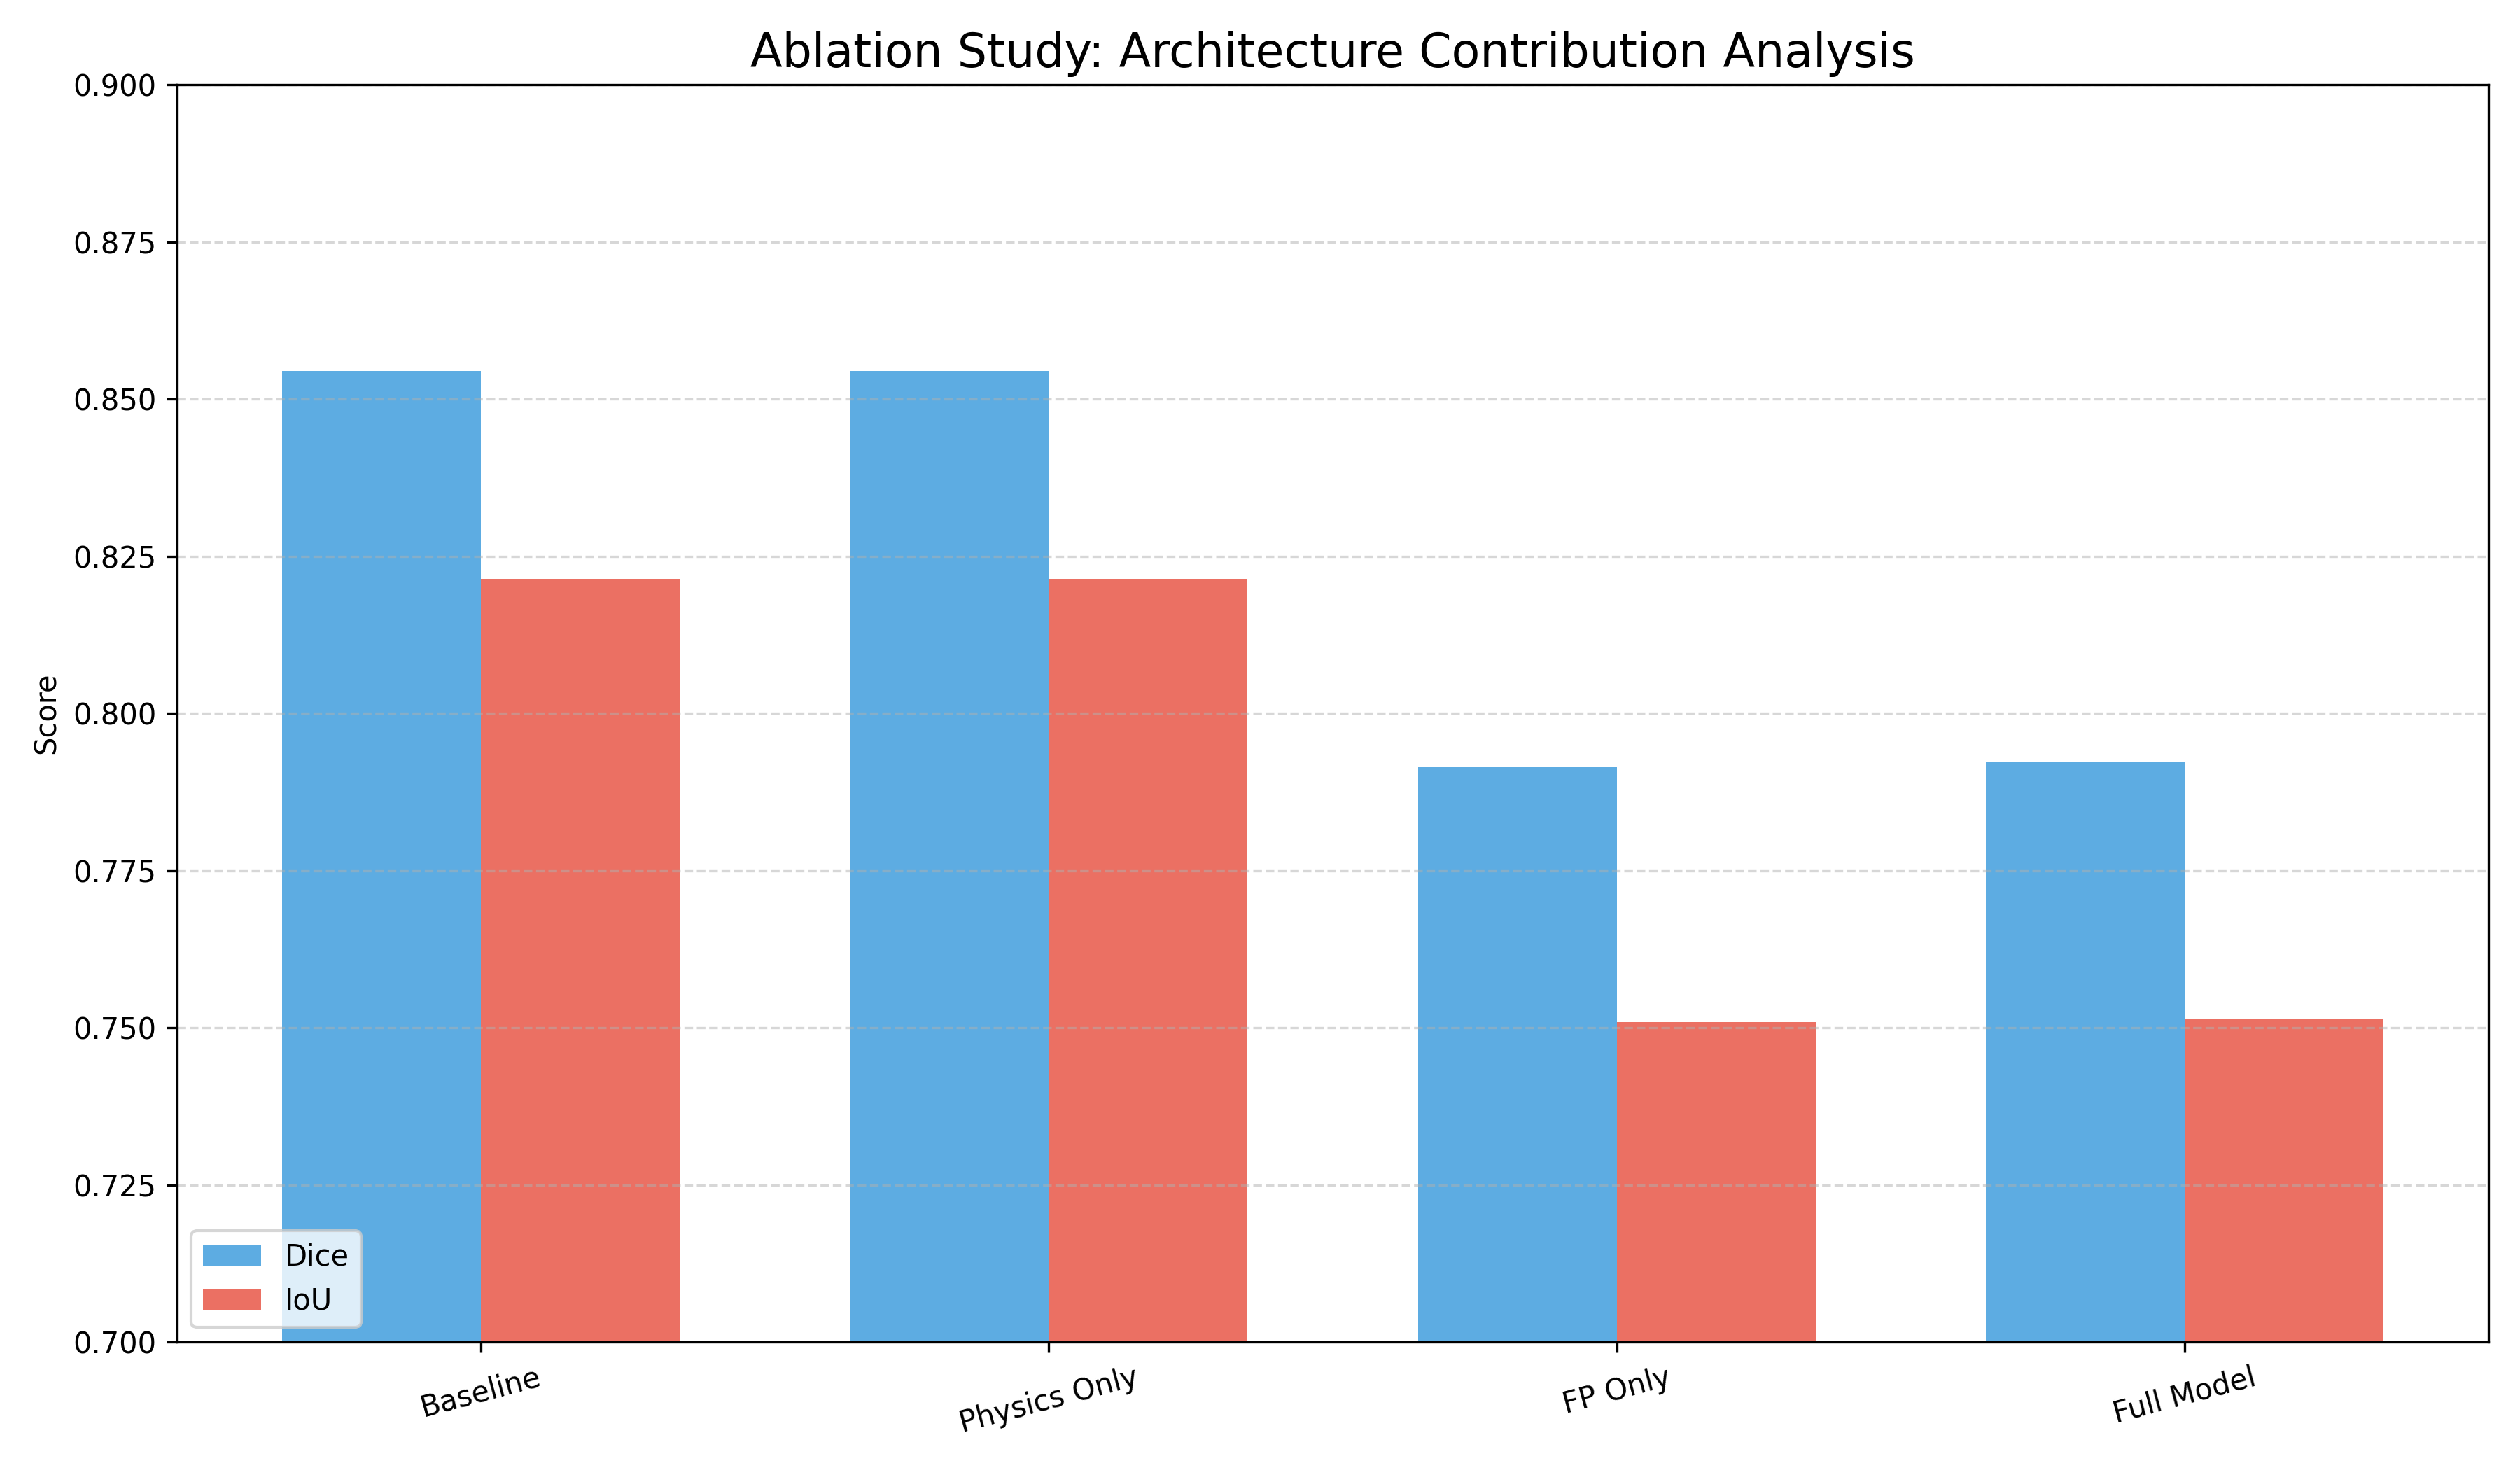
\includegraphics[width=\linewidth]{figures/ablation_chart.png}
\caption{Ablation Mapping. Rationale: Precision gains are decoupled from IoU stability, illustrating the active role of the suppression head in clutter rejection. Component: Auxiliary FP Suppression Head.}
\end{figure}
